\documentclass[12pt,openany,a4paper]{book}
\usepackage{graphicx}	% if you want encapsulated PS figures.
\usepackage{wrapfig}
\usepackage{verbatim}
\usepackage[hidelinks]{hyperref}
\usepackage{siunitx}
\usepackage{amsmath}
\usepackage[skip=2pt]{caption} % Bring captions closer to figure

% Rename bibliography to reference
\usepackage[nottoc,notlof,notlot]{tocbibind} 
\renewcommand\bibname{References}

\usepackage{cite}

\graphicspath{{imgs/}}

% Number subsections but not subsubsections:
\setcounter{secnumdepth}{2}
% Show subsections but not subsubsections in table of contents:
\setcounter{tocdepth}{2}

\pagestyle{headings}		% Chapter on left page, Section on right.
\raggedbottom

\setlength{\topmargin}		{-5mm}  %  25-5 = 20mm
\setlength{\oddsidemargin}	{10mm}  % rhs page inner margin = 25+10mm
\setlength{\evensidemargin}	{0mm}   % lhs page outer margin = 25mm
\setlength{\textwidth}		{150mm} % 35 + 150 + 25 = 210mm
\setlength{\textheight}		{240mm} % 

\renewcommand{\baselinestretch}{1.2}	% Looks like 1.5 spacing.

% Stop figure/tables smaller than 3/4 page from appearing alone on a page:
\renewcommand{\textfraction}{0.25}
\renewcommand{\topfraction}{0.75}
\renewcommand{\bottomfraction}{0.75}
\renewcommand{\floatpagefraction}{0.75}

% AIDS TO CROSS-REFERENCING (All take a label as argument):
\newcommand{\eref}[1] {(\ref{#1})}		% (...)
\newcommand{\eq}[1]   {Eq.\,(\ref{#1})}		% Eq.~(...)
\newcommand{\eqs}[2]  {Eqs.~(\ref{#1}) and~(\ref{#2})}
\newcommand{\dfn}[1]  {Definition~\ref{#1}}	% Definition~...
\newcommand{\thrm}[1] {Theorem~\ref{#1}}	% Theorem~...
\newcommand{\lem}[1]  {Lemma~\ref{#1}}		% Lemma~...
\newcommand{\fig}[1]  {Fig.\,\ref{#1}}		% Fig.~...
\newcommand{\tab}[1]  {Table~\ref{#1}}		% Table~...
\newcommand{\chap}[1] {Chapter~\ref{#1}}	% Chapter~...
\newcommand{\secn}[1] {Section~\ref{#1}}	% Section~...
\newcommand{\ssec}[1] {Subsection~\ref{#1}}	% Subsection~...

% AIDS TO FORMATTING:
\newcommand{\teq}[1]	{\mbox{$#1$}}	% in-Text EQuation (unbreakable)
\newcommand{\qed}	{\hspace*{\fill}$\bullet$}	% end of proof

% MATHEMATICAL TEMPLATES:
% Text or math mode:

% ORDINAL NUMBERS:
\newcommand{\ith}	{\ensuremath{i^{\rm th}}}
\newcommand{\jth}	{\ensuremath{j^{\rm th}}}
\newcommand{\kth}	{\ensuremath{k^{\rm th}}}
\newcommand{\lth}	{\ensuremath{l^{\rm th}}}
\newcommand{\mth}	{\ensuremath{m^{\rm th}}}
\newcommand{\nth}	{\ensuremath{n^{\rm th}}}

% NB: These have not been tested since being modified for LaTeX2e.
\newcommand{\pack}	{\hspace{-0.08em}}
\newcommand{\Pack}	{\hspace{-0.12em}}
\newcommand{\Hz}	{\ensuremath{\rm\,H\pack z}}
\newcommand{\cm}	{\ensuremath{\rm\,cm}}
\newcommand{\s}		{\ensuremath{\rm\,s}}
\newcommand{\ms}	{\ensuremath{\rm\,m\pack s}}
\newcommand{\us}	{\ensuremath{\rm\,\mu s}}

\begin{document}

\frontmatter
% By default, frontmatter has Roman page-numbering (i,ii,...).

\begin{titlepage}
\renewcommand{\baselinestretch}{1.0}
\begin{center}
\vspace*{35mm}
\Huge\bf
		Evaluating frame-based \\
        networks with temporal surfaces \\
\vspace{20mm}
\large\sl
		by\\
		Joshua Arnold
		\medskip\\
\rm
		School of Information Technology and Electrical Engineering,\\
		The University of Queensland.\\
\vspace{30mm}
		Submitted for the degree of\\
		Bachelor of Engineering
		\smallskip\\
\normalsize
		in the field of Software Engineering
		\medskip\\
\large
		June 2016.		
\end{center}
\end{titlepage}

\cleardoublepage

\begin{flushright}
	ADDRESS LINE 1\\
	ADDRESS LINE 2\\
	Tel.\ (07) nnnn nnnn\\
	\medskip
	\today
\end{flushright}
\begin{flushleft}
  Prof Michael Bruenig\\
  Head of School\\
  School of Information Technology and Electrical Engineering\\
  The University of Queensland\\
  St Lucia, Q 4072\\
  \bigskip\bigskip
  Dear Professor Bruenig,
\end{flushleft}

In accordance with the requirements of the degree of Bachelor of
Engineering in the division of 
Electrical Engineering,
Electrical and Biomedical Engineering,
Electrical and Computer Engineering,
Software Engineering,
Mechatronic Engineering,
I present the
following thesis entitled ``Analysing time-stepped neural networks with temporally rich frame-based data''.  This work was performed under the supervision of Prof. Janet Wiles.

I declare that the work submitted in this thesis is my own, except as
acknowledged in the text and footnotes, and has not been previously
submitted for a degree at The University of Queensland or any other
institution.

\begin{flushright}
	Yours sincerely,\\
	\medskip
	\emph{}\\
	\medskip
	Joshua Arnold.
\end{flushright}

\cleardoublepage

% Dedication (if you want it):
\vspace*{70mm}
\begin{center}
\renewcommand{\baselinestretch}{1.0}
\sl
	To \ldots
\end{center}

\chapter{Acknowledgments}


Acknowledge your supervisor, preferably with a few short and specific
statements about his/her contribution to the content and direction of
the project.  If you collaborated with another student, acknowledge
your partner's contribution, including any parts of the thesis of
which s/he was the principal author or co-author; this information can
be duplicated in footnotes to the chapters or sections to which your
partner has contributed.  Briefly describe any assistance that you
received from technical or administrative staff.  Support of family
and friends may also be acknowledged, but avoid sentimentality---or
hide it in the dedication.

\cleardoublepage

%%%%%%%%%%%%%%%%%%%%%%%%%%%%%%%%    ABSTRACT    %%%%%%%%%%%%%%%%%%%%%%%
\chapter{Abstract}

Event-based sensing offers many advantages in the field of artificial vision however few algorithms are able to leverage temporal aspect of the data fully. 
This deficit is due to a disparity between traditional frame-based algorithms developed for 2D images and the asynchronous nature of event-based data. 
A new event-based dataset of linear movement is presented and then used to evaluate the representational power of 2D temporally accumulated images in several shallow frame-based neural networks. 
%By retaining a time based blur in training data, frame-based networks are able to implicitly encode for temporal information in predictions showing 
By retaining a time based accumulation in training data, frame-based networks are able to make meaningful predictions which implicitly encode temporal information. 

\tableofcontents

\listoffigures

\listoftables

\cleardoublepage

\mainmatter
% By default, mainmatter has Arabic page-numbering (1,2,...).

\chapter{Introduction}

%The introductory chapter describes the importance of the field and the
%scope and significance of your project.  It usually ends with an
%overview of the remainder of the thesis.

%Notice that Arabic page numbering begins with Chapter 1.  Preceding
%pages (known as ``frontmatter'') have Roman numbering.  The
%\texttt{book} document class in \LaTeX\ follows this numbering
%convention by default (see Lamport~\cite{lamport}, p.\,80).





%% Broard intro to topic, where did this come from, what is the problem, 
Vision is the primary sense used by many natural agents to gather information about their environment.
It would seem to follow that vision should be an important percept for artificial agents.
%It would seem to follow that artificial agents should also be able to leverage visual sensors in a similar way.
% TODO Is digital systems the right term to use here??
However the apparent ease with which natural systems process visual information does not translate to standard digital arcitectures, making vision a seldom used sense. 
In real time applications vision is often impractical due to the computational load required to extract meaningful information. 
%In its place alternatives such as Infra-red for distance sensing or L.I.D.A.R. for mapping are substituted.
% TODO gonna need a refernce below
In a more theoretical environment there are still many challenges in extracting meaningful information from standard vision data due to variations in lighting, orientation, position, scale etc.


%% Breif into to neural nets
%   Why they are better than hard coded rules -> they can learn
A simplistic approach to vision processing would entail defining exact features of the object to be recognised.
This would quickly become overwhelming though as the system decends into considering a seemlingly endless list of special cases and permuations that a single object could take in an image.
% TODO will need a reference to standad analysis algoithms
%Numerous algorithms and heuristics have emerged making meaningful analysis possible in some circumstances such as ****** Color filtering / normal face detection?? / Canny edges? *******.
%Unfortunately these struggle to generalise to arbitrary object classification or prediction.
% TODO reference some state-of-the-art networks
%A promising alternative, Neural Networks, currently have state-of-the-art performance on many of the public benchmark datasets.
Alternatively an algorithm designed to detect a specific object using heuristics or traditional vision processing methods could be used.
Unfortuneately these only solve a smaller part of the processing problem, such as canny edge detection, or struggle to generalise to objects other than that they were designed for, such as ** face detection **.
Neural networks offer a general solution to the problem of classification and prediction.
Rather than relying on expertly designed heuristics or algorithms a neural network is randomly initialised and after repeated presentations of some stimuli can adjust internal parameters to minimise a loss function. 
This ability to self adjust and decide which parts of the stimuli are important has lead to systems capable of learning representations far more complex than an expert would have been able to design explicitly. 


Breif into to Event-based sensors \hfill 
   fast, low power, sparse, biologically realistic \hfill

Why the DVS with NN's makes sense \hfill 

\textbf{[TODO: finish off intro once I know the structure of everything else...]}
%\section{}
             % 3
\chapter{Literature - Sensors, Processing, Networks}

%%%%%%%%%%%%%%%%%%%%%%%%%%    ASYNC SENSORS     %%%%%%%%%%%%%%%%%%%%%%%%%%%%%%%%%

\section{Asynchronous Vision Sensors}  % 1 page
%Lots of different types of dynamic vision sensors \cite{delbruck2010activity}
%Why would we want a DVS? microparticle tracking \cite{ni2012asynchronous}
%Neuromorphic systems are becoming more wide spread \cite{delbruck2014research}
% Introduction to AVS 
%Introduce different kind of senssors which asynchronously fr
Asynchronous Vision Sesnors (AVS) offer a frame--free, event--driven approach to capturing vision information\cite{delbruck2010activity}. 
These sensors continuously output light intensity changes from a scene in the form of precisely timed (sub \ms) events. 
Each pixel in the sensor array acts independently based on the light in its receptive field resulting in a sparse, stimulus--based output. 
A recent spike in technology facilitated the development of many alternative asynchronous vision sensors with varying properties and speeds\cite{delbruck2014research}.
These systems are united in an attempt at emulating the efficient, high--speed, event--based spiking behaviour in biological vision systems\cite{delbruck2010activity}.
%Environments requiring low-power, low-latacy and dynamic range are well suited 
Asynchronous vision sensors are well suited to environments requiring dynamic range, low-power and low--latency sensing, such as microparticle tracking\cite{ni2012asynchronous}, robotics\cite{roboGoalie2013} or motion tracking and classification\cite{Lee2014, reverter2015neuromorphic}.

% How do they work
In contrast to traditional vision systems which densely sample the world at discrete time intervals, AVSs follow a stimulus driven paradigm only recording changes in the environment, meaning redundant information in the scene (e.g. stationary items or backgrounds) are not captured.  
The resulting data format, Address-Event Representation (AER)\cite{mahowald1992vlsi}, is in the form $\textless (x, y), t, p \textgreater$, where $(x, y)$ is the pixel location of a change, $t$ is the precise time of the change and $p$ is the polarity indicating if the light intensity change was brighter (positive event) or dimmer (negative event)i\cite{delbruck2010activity}. 
% TODO really should find a AER specific paper for this
This dramatically different data representation means new approaches to vision processing will be required to extract meaningful information from AER sensors\cite{akolkar2015can}. 

% They why. What are the advantages and disadvantages
Asynchronous vision sensors offer a new paradigm in which to approach capturing vision information, bringing with it many new opportunities and challenges. 
The low--redundancy asynchronous nature of these sensors allows low--power, low--computation processing in a more biologically realistic setting.



\subsection{Example sensors}
%Tobi made a camera \cite{delbruck2008}
%Discuss the Dynamic vision sensors, what they are capable of
%Used in stuff like \cite{delbruck2007fast}
%They also have a new camera called the DAVIS \cite{DAVIS}
The Dynamic Vision Sesnor (DVS) is an AVS capable of registering events to temporal precision of 15\us\cite{delbruck2008}. 
It has a 128x128 pixel array with \textgreater 120\textit{dB} dynamic range.
The Dynamic and Active Pixel Vision Sensor (DAVIS) is the newer model of the DVS with a 240x180 pixel array, 3\us temporal precision and 130\textit{dB} dynamic range\cite{DAVIS}. 
Additionally the DAVIS has circuitry (the active pixel sensor) enabling it to capture static scene illumination values like a standard camera.
Further an inbuilt inertial measurement unit (IMU) means movement information can be simultaneously recorded and used in processing. 
An alternative sensor is the asynchronous time-based image sensor (ATIS) with a temporal resolution of 10\us (at \textgreater100Lx)\cite{posch2011qvga}.
Like the DAVIS the ATIS is also capable of capturing scene illumination as well as events.  





%%%%%%%%%%%%%%%%%%%%%%%%    STANDARD VISION     %%%%%%%%%%%%%%%%%%%%%%%%%%%%%%%%%
\section{Frame-based vision processing}   % 1 page
%Standard videos and frame based approaches

% Introduction to standard vision processing 
Standard vision processing has long been based on processing full 2D frames using well understood techniques such as Canny Edge detection\cite{canny1986computational}. 
Many techniques exist for various tasks such as face detection\cite{viola2004robust}, object tracking using kernels\cite{comaniciu2003kernel} or object classification\cite{krizhevsky2012imagenet}.
The method of these approaches varies significantly from gradient based computation in Canny Edge detection to kernel based object tracking to deep neural networks.
Yet they all make the same implicit assumption that vision information is temporally discretised into the frame-rate of the vision sensor used in recording. 

Frame-based techniques and associated applications are thus bound by the limitations of the recording device with respect to data speed and quality. 
In particular if a standard 30 fps camera is used a realtime system must wait 33ms between frames (excluding any processing time required). 
Using a higher frame--rate recording device has a bound on performance as this necessarily means there will be more data (much of which is redundant) to process, such that the processing time of the system becomes the bottle neck. 
Further image quality in frame-based systems is proportional to the amount of processing required to extract features.
Despite limitations from recording devices, many impressive results have come from these techniques, in particular deep neural networks\cite{krizhevsky2012imagenet}.
However the computation required for these state-of-the-art systems makes their use on low--power, low--computation devices impractical. 



%%%%%%%%%%%%%%%%%%%%%%%%    EVENT-BASED PROCESSING     %%%%%%%%%%%%%%%%%%%%%%%%%%%%%%%%%
\pagebreak
\section{Event-based processing}     % 2 page
% Intro to what event based processing is (using events)
Event-based data brings with it the need for radically different processing paradigms compared to frame-based approaches\cite{perez2013mapping, martin2015spiking, tan2015benchmarking}.
Conventional sensors generate large amounts of redundant data which is computationally expensive to process, making efficient event-based data an attractive option\cite{vanarse2016review}. 
Event-based processing is not limited to vision sensors however, as discussed in \cite{vanarse2016review} neuromorphic auditory and olfactory sensors also exist using the AER format. 
Challenges facing event-based vision sensors are shared among these other neuromorphic sensors as well as more common (and low cost) sensors (like IMUs for gait cycle measurments\cite{fida2015pre}).

Many standard machine learning techniques have implicit assumptions that data is discretised into uniform time samples or that temporal information is not present/important.
There have been attempts to integrate temporally rich data with standard frame-based approaches such as the recurrent Temporal Restricted Boltzmann Machine (TRBM)\cite{sutskever2009recurrent} to model motion capture data or using deep-belief networks with spiking systems\cite{Neftci2014, pedroni2013neuromorphic, OConnor2013}.
More suited to dealing with event-based data are the family of Spiking Neural Networks (SNN)\cite{henderson2015spike, perez2013mapping}.
SNNs are harder to train than the frame-based counterparts, leading many to train frame-based networks and convert the trained model into an equivilant spiking network at some small performance drop\cite{perez2013mapping, pedroni2013neuromorphic, OConnor2013}.

Event-based processing is not limited to neural networks and other techniques are being adapted or created to take advantage of these new highspeed sensors\cite{ni2015visual}.
A \textit{RoboGoalie} was created as an example application leveraging the low-latency sensor to stop fast moving ping-pong balls entering a goal\cite{delbruck2007fast}. 
A simple event clustering algorithm was sufficient to allow the RobotGoalie to track incoming balls and respond within 3\ms with a peak performance load of 4\% on a standard computer. 
This was conducted in a heavily constrained system though, where luminance was controlled, the DVS stationary and with a constant background. 
Strict weight, power and computational requirements of a quadrotor form a near-perfect environment in which traditional cameras fail and event-based sensors shine\cite{mueggler2014event}.
These low-power and low-computation features of event-based sensors make them particularly attractive for applications in mobile robotics and navigation\cite{weikersdorfer2013simultaneous, milford2015place}.
These constraints have led to focused efforts on developing efficent algorithms to calculate odometry \cite{censi2014low}, visual flow \cite{benosman2014event} and corner detection\cite{clady2015asynchronous}.

% More on applications here then next para will support why they make sense

The systems described have shown that through careful datastructures and representations, learning models are able to leverage temporal information from the precise spike timings of event-based data. 
It is well known the eye does not act as a traditional vision sensor capturing and transfering full frames to the brain but rather sends only relevant visual information in the form of spikes\cite{delbruck2010activity}.
In an attempt to mimic this spiking behaviour some have attempted to convert frame-based benchmark datasets into spiking equivilants using grayscale values to produce rate-coded spiking outputs, while others have suggested why this may be problematic \cite{akolkar2015can} and suggest guidelines to ensure dataset quality\cite{tan2015benchmarking}.
Studies have found that coding schemes using the precise timing of events may be more biologically realistic and account for situations where processing happens too quickly to be explained by rate-coded information transfer\cite{thorpe2001spike}. 
It was similarly found that the precise spike timings of events in event-based data has a significant contribution to the amount of information contained in the recording\cite{akolkar2015can}.
% NOTE: Thus precise spike timings are important so maybe using a screen is bad. 


%What other processing has already been done with them (things like Motion cones). 
%Example usage of DVS is fast motor control by \cite{delbruck2007fast}
%Discuss frame accumulation by other groups
%Example of event-based visial flow calculation by fitting local plans on incoming events\cite{benosman2014event} (what else is this lab doing?)
%Calculating odometry using event based information (application) \cite{censi2014low}
%event-based corner detection\cite{clady2015asynchronous}


\subsection{Visual information representations}

% The eye can process well
The ease with which biological systems can process visual information suggests it should be a key percept in artificial agents, but it is not.
% But uses funny data formats
The challenges limiting artificial vision systems may be in part due to the fundamental differences between the biological equivilant in both recording and data format.
% DVS is like the eye
Neuromorphic vision sensors have started to emerge closing the gap between artificial systems and biology\cite{mahowald1992vlsi}.
% and has similar data formats
These sensors record and output data which much more closely resembles the retina\cite{akolkar2015can}. 
% Could convert to Frames
Although more biologically realistic, the data formats from these sensors are fundamentally different to frame-based representations prohibiting standard processing techniques. 
Converting between events and frames can be as simple as collecting all events from a time period into a frame as in \cite{kogler2009bio, schraml2010dynamic} or involve more complex calcuations about the events usefulness\cite{mueggler2015lifetime}.
Inversely, there has been work converting from frames back to realistic spike-train\cite{afshar2013ripple} showing this conversion is not a simple mapping but contains losses\cite{akolkar2015can}. 
%   Not-bio but it works
Accumulating events into frames works with current processing paradigms but departs from biology which is likely using precise neuron firings as representations\cite{akolkar2015can}.
% If we want to process well we must learn to process data formats too
To achieve biological system level performance is may be necessary to preserve additional qualities of the biological data format and processing. 
% We have AER
Perhaps the most biologically realistic format considered for processing is the AER format \cite{mahowald1992vlsi}.
%   But this is limited in number algorithms
This relatively new format has few algorithms that can fully leverage the structure, some worthy mentions include a high-speed pencil balancing robot \cite{conradt2009pencil}, a robotic goalie \cite{roboGoalie2013} and scene reconstruction with super-pixel resolution\cite{kim2008simultaneous}.
%   Could use Spiking neural networks (but hard to train)
% Temporal surface
A middle ground between direct frame accumulation and AER formats is the use of a short term window in which events have some influence.
Memory surfaces are present in the literature in forms such as gaussians approximating position \cite{conradt2009pencil}, queues of events \cite{ni2012asynchronous} or as this work will investigate, functions of temporal difference \cite{afshar2016investigation}.


% 

%Disucss how this is more like the eye and the advantages of this model of processing \cite{mahowald1992vlsi}

%Interest in event-based processing and sensors stems from the analogies to biological vision and processing\cite{mahowald1992vlsi}. 
%Necessarily vision sensors more like biological retinas must use  essence of neural processing data structures which closely resemble real .

%Rumelhart's back prop might not actually be biologically realistic but effective in learning regardless \cite{Rumelhart1986}.
%Discusses the biological realism of using spikes \cite{akolkar2015can}
%What does this paper say about representations maybe bio isn't always an answer \cite{fida2015pre}

%Temporal surfaces \cite{afshar2016investigation}



%%%%%%%%%%%%%%%%%%%%%%%%%%%%%%  NEURAL NETWORKS   %%%%%%%%%%%%%%%%%%%%%%%%%%%%%%%

\section{Neural Networks}     % 1 page
% Neural networks are loosely based on the brain
Artificial neural networks have origins as software implementations of brain functions\cite{mcculloch1943logical}.
Several seminal breakthroughs, notably backpropagation (popularised by \cite{Rumelhart1986}), convolutional neural networks \cite{lecun1998gradient} and more recently deep learning \cite{schmidhuber2015deep} have made neural networks a powerful tool in many learning tasks. 
% Impressive performance (state of art) in image classification
In particular neural networks have become the state-of-the-art in many image recognition and classification tasks \cite{krizhevsky2012imagenet, szegedy2015going}.

% Composed of layers of processing units (neurons)
Artificial Neural networks are made up of many processing units (neurons) each which does a small computation and produces output. 
% Type and function of units affects network dynamics
The function that each individual processing unit computes can have a significant affect on the network performance (measured by a loss function). 
%   perceptron
The first, and perhaps simplest, processing unit is the perceptron which computes a binary classification based on whether a weighted sum of inputs excedes a threshold.
Perceptrons represent a simple base line from which to compare other unit activation functions.
Learning with a binary output can be troublesome and perceptrons can be augmented to accept real valued input and give real valued output.
These augmentations means the units will compute a linear function of the input.
%   Sigmoid
%More complex, non-linear, functions may be necessary in a le
Many challenging tasks cannot be solved using a linear transformation of the input leading to more complex, non-linear, activation functions being used.
In particular sigmoid (along with other bounded, nonconstant) activation functions have been shown to be universal approximatiors\cite{hornik1991approximation}.
%   ReLU
More recently Rectified Linear Units (ReLU) have become a popular non-linear unit\cite{lecun2015deep} for the faster training times and biological realism compared to sigmoid units \cite{glorot2011deep}.
%   More complex LSTM units exist but not used
Even more complex units with special properties such as memory in Long Short Term Memory units \cite{hochreiter1997long} could be used to keep a state in the network. 

% Specifying weights impossible so we use back prop and SGD to refine weights
%Adjusting internal parameters of the network cause it to compute different functions on the input, its performance can then be evaluated according to some loss function. 
A network simply computes some function on input producing output, for the network to solve a task the weights of each unit need to be set appropriately.
Setting these weights using human experts would not be possible due to complexity and number of units.
Instead learning rules can be used to adjust the weights in the network based on the networks performance on training examples (input and output pairs). 
% Loss functions play a big role
The network's performance on any given training example is measured by a loss function which the learning rule aims to minimise. 
A widely used learning rule is Stochastic Gradient Descent (S.G.D.) which adjust weights based on computing the steepest gradient using the backpropogation algorithm\cite{Rumelhart1986}.


\subsubsection{Autoencoders}
% What they do and how they work to clean data/form representations
Autoencoders are typically feed forward neural networks tasked with finding efficient data codings\cite{hinton1994autoencoders}.
A simple structure entails a single hidden layer which converts an input into a compressed code.
The activations of the hidden layer can then be converted back into a representation of the input through the weights of the output layer.  
That is, the input and output are identical so the network must learn to encode the dataset with the units in it's hidden layer. 
These networks are also useful for denoising datasets and dimensionality reduction\cite{hinton2006reducing}.


\subsubsection{Convolutional networks}
% Use in image processing 
Loosely analogous to receptive fields found in mammalian visual systems \cite{hubel1962receptive, hubel1968receptive}, units in convolutional nerual networks can focus on small spatial regions of the input for specific features. 
In standard networks weights must be specialised to extract a particular feature from a given location in an image.
If the weights have specialise and the input undergoes a spatial translation the weights will no longer be able to effeciently extract the feature.
Convolutional networks develop specialised visual feature detectors and use them repeatedly in a grid like pattern across the input to extract information\cite{lecun1998gradient}. 
This translational invariance means convolutional networks can create more feature detectors for the same number of weights as a standard network.
Using feature detectors in this way allows networks to ignore parts of the input while focusing on the current area. 
%Networks are also able to ignore background noise in an input and 
%By using the same feature detector at different locations on the same input commonly occuring features can be extracted from different spatial locations without the need for repeated weights 

%\subsection{Deeper networks}   % 1 page
%ResNet etc. % TODO find resnet reference
%ImageNet etc.
%This was some deep network work \cite{pedroni2013neuromorphic}
%Oconor used deep networks \cite{OConnor2013}

%\subsection{Spiking networks}    % 1 page
%O'Connors work on spiking deep belief networks \cite{OConnor2013}
%Using echo state networks to extract spatiotemporal features from event-based \cite{lagorce2015spatiotemporal}
%Move to spiking networks accompanied by converstions from 2D to 1D temporal trains \cite{afshar2013ripple}
%Discussion on 2D images and converting to spikes vs just using spiking sensor and the information preserved \cite{akolkar2015can}
%Paper on spiking networks for vision tasks, usese the DVS and compares to convNets \cite{martin2015spiking}
%Feeding a DVS output directly into spiking NN \cite{Bichler}
%Interesting learning rules for SNNs \cite{Bichler} not exaimined here though.

\subsection{Software frameworks}   % 1 page
Many software frameworks exist for implementing and running neural networks including; Caffe\cite{jia2014caffe}, Theano\cite{bastien2012theano}, Torch7\cite{collobert2011torch7} and Tensorflow\cite{abaditensorflow} plus many more.

\textbf{Caffe} is a deep learning framework created by the Berkeley Vision and Learning Center and released with a BSD 2-Clause license.
Caffe has GPU support, API's for the command line, python and matlab while underlying code base consists of C++ and CUDA.
Network structure and parameters are specified in Google's Protobuf format as Directed Aycyclic Graphs.

\textbf{Theano} is an python based computation library for mathmatical expressions that works closely with Numpy multi-dimensional arrays.
Networks are defined in python as computation graphs which can then implicitly use underlying C implementations or GPU routines for calculations. 
Theano is relased with a BSD 3-Clause license.

\textbf{Torch7} is a compution framework with a focus on GPU computation.
Calculations are specified in the LuaJIT programming language and calculations are done with underlying C and CUDA implementations. 
Torch7 is released under the GNU Public License.

\textbf{Tensorflow} is Google's numerical computation library with a focus on support for many different systems including CPU, GPU, mobile and embedded systems.
Computation graphs are specified in Python while calculations are done with underlying C and CUDA implementations. 

All of these frameworks have the required functionality for this project.
Theano and Torch7 have been competing for faster processing times \cite{bergstra2010theano, collobert2011torch7, bastien2012theano} in recent years securing them both processing times better than Tensorflow or Caffe\cite{bahrampour2015comparative}.
However as only shallow neural networks will be used optimised performance is not strictly needed.
Caffe requires a complex installation of many components/libraries and uses a less intuative model specification (protobuf). 
Torch7 also uses the less standard LuaJIT for model specification.
Tensorflow was indentified as the slowest but also as the most flexible framework.

\section{Neural Networks with event-based data}
With some exceptions, neural networks map a set of inputs to a set of outputs.
% Doesnt mesh well with DVS data
This paradigm does not mesh well with event-based data which has no natural segments to use as inputs as frame-based vision has frames. 
% Need different ways to incorporate the data 
Many different appraoches have been taken to convert event-based data into a format the network can accept but perhaps the most natural is the use of spiking neural networks. 
% We could try spiking nets naturally these make sense, oconnor, spiking convs and Amy
Unlike frame-based neural networks spiking neural networks use the timing of input to transfer information \cite{akolkar2015can}.
A set of spikes is called a spike train and spiking neural networks can learn to differentiate between individual or collections of spike trains. 
% Contrastive divergence (spiking version as well)
Despite this suitability for event-based data spiking neural networks are harder to train and require different learning rules \cite{walter2015neuromorphic, henderson2015spike}.
Some notable work converted a fully trained, frame-based, deep belief network into an event-based spiking neural network with less than 1\% drop in performance\cite{OConnor2013}. 
% Saeed convert from spiking to feature maps
%Using event-based data and feeding it into a network (Saeed) \cite{afshar2016investigation}
Alternatively spiking networks have been used as just a part of the processing to extract meaningful features before using a standard network for classification\cite{afshar2016investigation}.
Work has also been done trying to convert frame-based techniques like contrastive divergence \cite{Neftci2014} or backpropagation (SpikeProp) \cite{bohte2002error}.
Specific spike-based algorithms for extracting features from event-based sensors also exist \cite{Bichler} but are much less common than frame-based methods. 


\subsection{Benchmark datasets}
To fairly compare models it is necessary for the community to have standardised datasets\cite{barranco2016dataset, Gibson2014, tan2015benchmarking}.
Many datasets exist for frame-based models from well formatted and normalised datasets (such as MNIST\cite{lecun1998gradient}) to large complex datasets (such as ImageNet\cite{deng2009imagenet}).
In an attempt to compare event-based processing models to frame-based models some have used DVS recordings of the classic MNIST dataset, being either with stationary images and a moving sensor \cite{OConnor2013, orchard2015converting} or with a sationary sensor and moving images on a screen \cite{serrano2015poker, akolkar2015can}.
Notably different to others is the secondary digit dataset in \cite{akolkar2015can} in which a DVS performs vertical saccades while recording digits on a rotating cylinder.
However, in trying to be comparable with frame-based models these datasets fail to realise the full potential of the DVS to capture complex spatio-temporal surfaces because the simulus is inherently two dimensional.
Newer benchmark datasets have addressed this problem offering a wide range of stimuli, in particular complex real world self motion for a mobile robot \cite{Gibson2014, barranco2016dataset}.
There is still a deficency of extremely simple datasets around which strong foundations can be formed to allow a deeper understanding of network dynamics.
Further as capturing movement is a key advantage of the DVS over frame-based sensors this should be emphasised in datasets.


%Creates own plane dataset \cite{afshar2016investigation}

%%%%%%%%%%%%%%%%%%%%%%%%%%%%%%%%%    SUMMARY    %%%%%%%%%%%%%%%%%%%%%%%%%%%%%%%%%%%%%

\section{Literature summary}      % 1 page
%Revisit each section in a sentance or two and link them all together.
Asynchronous
% Asynchronous vision sensors, summarise pos, neg and diff and motive why we look at them
% This work will only use the DVS
% Standard vision processing has come a long way and has good techniques but bad assumptions
% Event-based data is dramatically different
    % Doesnt work with standard vision techniques
% We can try and convert from DVS to frames but need to be careful 
% Neurel networks are awesome at processing so lets use those, 
    % We should try different activations
    % should try different structures, convolution for its bio inspired ness
    % We might also be able to use networks to clearn the data (autoenc)
    % Several software frameworks examined, gonna use tf 
% A sensible apparoch to evnet-based is spiking nets but lets use frame-based anyways
% But before we get started lets see what kind of datasets already exist for us to use...








%Evolving probabilistic spiking neural networks for spatio-temporal pattern recognition: A preliminary study on moving object recognition \cite{kasabov2011evolving}

Neuromorphic adaptations of restricted boltzmann machines and deep belief networks, These guys (in particular Pedroni) had something stuff \cite{pedroni2013neuromorphic}


Double check the use of this paper \cite{gil2014active}

How does this paper fit? applications? what are they doing? temporal surfaces maybe? \cite{davide2014high}

again high speed object tracking (diff authors) \cite{saner2014high} 

More somewhat unrelated, must just use about the methods of processing \cite{mueggler2015continuous}
         % 12
\chapter{Datacollection}

\section{The need for a dataset}
To fairly compare models it is necessary for the community to have standardised datasets (REF MNIST, CIFAR ETC.). % Reference MNIST, CIFAR etc.
Many datasets exist for time-stepped models from well formatted and normalised datasets (such as MNIST) to large complex datasets (such as ***ImageNet dataset?***).
In an attempt to compare event-based processing models to time-stepped models some have tried using DVS recordings of static MNIST digits (REF O'CONOR). % ref OConor
However this doesn't capture the full potential of the DVS to capture complex spatio-temporal surfaces as the simulus is inherintly 2D.
Newer benchmark datasets have addressed this problem offering a range of stimuli, in particular complex real world self motion for a mobile robot (REF AMY PAPER). %% Ref Amy
There is still a deficency of extremely simple datasets around which strong mathmatical foundations can be laid to allow a deep understanding of network dynamics. 
As capturing movement is a key advantage of the DVS over time-stepped models this should be emphasised in the dataset. 
%This work offers such a dataset consisting of dots moving linearly with constant velocity. 

\section{Requirements and details for 8AD and AAD}
The motivations behind such a dataset must be carefully considered so when collected it forms a comprehensive set.
Simple structure is required so that when experimenting with new appraoches to processing dynamics in the system can be reasoned about with some accuracy.
Additionally a dataset for complex real world (robotic self-motion) or interesting patterns already exists, it is simpler data that is necessary.
To evaluate the accuracy of classification systems a ground truth is also required labelling events as signal or noise. 
With the advent of deep learning the advantages of large bodies of labeled training data have become apparent. 
Thus the ability to collect a large number of samples is also deemed necessary and the system should be as autonomous as possible. \\ 
\textbf{Final requirements:}

\begin{itemize}
    \itemsep-0.5em
    \item \textbf{Simplicity} -- To allow model analysis 
    \item \textbf{Movement} -- Key advantage of the DVS
    \item \textbf{Labels} -- To facilitate learning and validation
    \item \textbf{Autonomous} -- So large amounts can be captured
\end{itemize}

Considering the gap this dataset will fill and the requirements specified the simplest datum was decided to be a single dot moving linearly with a constant velocity. 
The variables to be manipulated include the dot diameter, velocity and direction. 
These variations recorded are listed in table \ref{tb:datasetspecs}.
As a stepping stone from simple datasets to more complex real world datasets two further variations were considered; two dots intersecting at the center of the screen and multiple dots tracing arbitrary angles (occationally intersecting).  

\begin{table}[h]
\centering
\begin{tabular}{ | c | l | }
    \hline
    Dot size (pixels) & 4, 6, 8 \\
    Angles (degrees) & [0 - 360] \\
    Starting position & Random \\
    Velocity (pixels/update) & 2, 4, 6, 8 \\
    \hline
\end{tabular}
\caption{Arbitrary Angle Dataset specification}
\label{tb:datasetspecs}
\end{table}

The above specification details what is from here on called the Arbitrary Angle Dataset (for berevity it will be referred to as AAD), that is, in this dataset the starting position of the dot does not restrict its direction.
An even simpler dataset from here on called the 8 Angle Dataset (for berevity, 8AD) is also presented in which the dot can only start from a corner of the screen or the middle of the one the edges.
The starting position of the dot also then dictates the direction the dot will move e.g. if it starts in the top left of the screen it must go to the bottom right or if it starts in the center of the top edge it must go to the center of the bottom edge.

% Okayyyy for 8AD lets run 250 of each angle 



%%%%%%%%%%%%%%%%%%%%%%%%%%%%       CONSIDERATIONS    %%%%%%%%%%%%%%%%%%%%%%%%%%%%%%%%%
\section{Considerations}
\subsection{Stimulus generators}
With clear requirements the practical generation of the dataset can be considered in detail.
The requirement for constant velocity would prove difficult to control in any real world system with forces of friction and gravity.
Such a real world system would also prove uneconomical in terms of time required to construct and, unless well automated, time required to conduct recordings. 
Recording computer simulations becomes an attracive option (particularly in regards to recording ground truths) but comes with its own negatives including screen refresh rates.
Recording from a computer screen also beings the disadvantage of non-continuous stimuli, the dot must be discretised, drawn onto pixels and thus screen pixel size forms the grid on which the stimuli is restricted. 
This issue can be mitigated when considering the much finer resolution of a screen compared to the DVS, the discretisation of the dot on a screen will have minimal effect if the dot is comprised of enough screen pixels.
The non-continuous stimuli issue can likewise be alliviated by restricting the dot movement to low velocities meaning in any given refresh of the screen the dot only moves by a small amount and thus approximates continuous movement. 


\subsection{Data quality concerns}
%Flashes on screen -> noise
%Light invariance
%Ground truth to actual recording consideration (mitigated through setup?)

The DVS's temporal resolution of \SI{15}{\micro\second} mean it should be able to detect screen refresh rates (every \SI{16}{\milli\second} on a 60Hz screen). 
It would be expected that every \SI{16}{\milli\second} there should activity across the whole sensor for a short time period. 
This does not seem to be the case with the DVS though, the same experiement run with the newer DAVIS sensor (with temporal resolution of \SI{3}{\micro\second} occationally is able to capture the screen refresh rate but even this is not consistant as show in figure \ref{fig:refreshFlashes}.

\begin{figure}
    \centering
    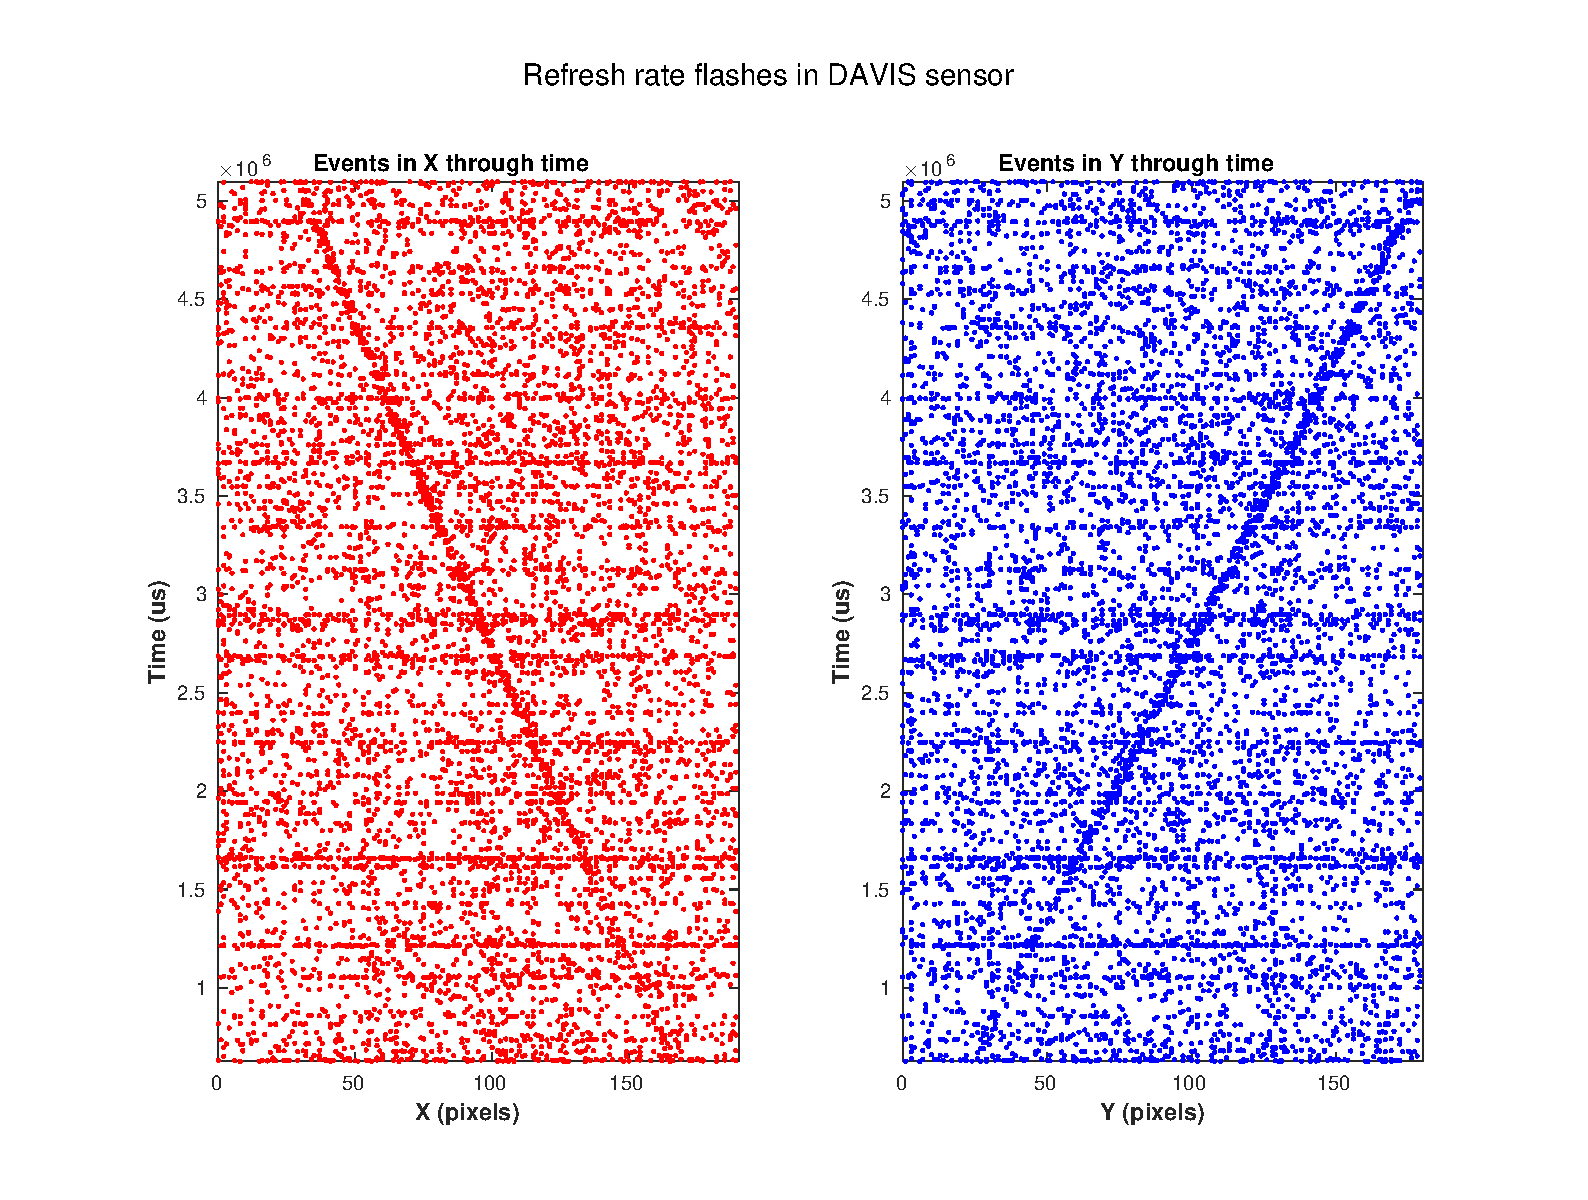
\includegraphics[width=0.8\textwidth]{screenFlashes.eps}
    \caption{Refresh rate flashes captured by DAVIS sensor}
    \label{fig:refreshFlashes}
\end{figure}

The DVS will only trigger and event if a pixels internal value has changed by 15\% meaning in low light situations the DVS will register an event more readily. 
Not all recording will be done in one session and changes to ambient light due to environmental conditions may have an impact on recording quality by triggering more or less events for the same stimuli.
This affect should be minimal if all recordings are done at roughly the same time of day in the same room with the same screen. 

A more serious concern is that of ensuring label consistency between the screen pixels and the DVS pixels. 
When recording from the screen it will be critical to ensure the DVS is carefully aligned with the edges of the stimuli.
Failure to align the two will result in labels being misleading as the recording will be offset.

\subsection{Processing considerations}
%Segmenting datasets
%Line angles (Close to edge, just a tiny segment in corner)
In an autonomous collection setup the question of data integrity must be raised.
Numerous situations could lead to the experiemental setup becoming compromised without experimenter knowledge such as the DVS being bumped.
Additionally in processing the data computer ground truth labels may accumulate an offset after many samples.
These problems can be avoided by embedding meta-data in the data recordings which keeps the processing transparent. 
The suggested meta-data to include is the trajectory of the line in this sample as well as a horizontal and vertical line crossing at the center of the screen.
This will allow callibration of the DVS's rotational and linear offset from the center of the stimulus as well as tracking of the dots path in this offset view. 
The full protocol for an experiment will thus be:

\begin{itemize}
    \itemsep-0.5em
    \item Flash dot trajectory (30\ms)
    \item Actual sample (dot following trajectory)
    \item Flash dot trajectory (30\ms)
    \item Flash cross (30\ms)
    \item Repeat for next dot and trajectory.
\end{itemize}

The process of flashing the dot trajectory, the cross and then the next dots trajectory will be referred to as a meta-flash. 
Using these meta-flashes means the data can be independently verified by other researchers and will produce a histogram of total number of spikes similar to figure *** Create and insert figure ****.
This makes segmenting samples a matter of extracting the regions in which the total number of events is below some threshold (which various proportially to the size of the dot, and hence the number of events it produces). 

%TODO figure as per figure 4 from proposal (showing use of meta-flashs).



In the arbitrary angle samples it will be possible for a dot to start close to a corner and to move to the adjacent edge resulting in a sample with a path of only a few (\textless 5) DVS pixels and lasting less than a second.
This case was considered troublesome for later processing steps and thus the starting points in the arbitrary angle dataset were restricted to the middle 80\% of each edge. 

\subsection{DVS curiosities}
%Black on white and white on black, grey
%Hot pixels

The DVS is still a new research tool and as such still has some peculiarities, in particular due to the manufacturing process some pixels, called 'hot pixels', in the array fire more frequently than others regardless of stimuli. 
These hot pixels are a source of noise in the data and could be removed in software or hardware but the effect is minimal compared with the standard noise of neuromorphic sensors so was left in these experiments. 

As mentioned when discussion lighting variations during experiments, DVS pixels will more readily fire if their internal value is smaller.
This has implications when the DVS is recording a black dot on a white screen or a white dot on a black screen.
The black screen means the DVS is more sucseptible to abient noise and will fire more events for a white dot, when compared to a black dot of the same size on a white screen. 
This phenomena is not expected to reveal any significant insight related to this thesis and is considered out of scope but its cause is worth considering whilst designing experiments. 



%%%%%%%%%%%%%%%%%%%%%%%%%%%          METHODOLOGY         %%%%%%%%%%%%%%%%%%%%%%%%%%%%%%
%TODO maybe this should just be a sub section since its so small, what else should go here?
\section{Methodology}
%What did i actually end up doing
The final system consisted of a program called dotGen written in python which would display the dot moving along a trajectory with meta-flashes.
DotGen also had tools to start a DVS recording, adjust dot parameters (size and velocity) and help set up the DVS correctly. 
DotGen would log the ground truth of the dots position to a CSV file in the format <x, y, time> every time the screen was updated.
The screen recorded from was a Dell U2414H Monitor with a refresh rate of 60Hz.
DotGen and jAER were started and the camera positioned to exactly capture the screen size then the recordings were taken. 




%%%%%%%%%%%%%%%%%%%%%%%%%%%         FINAL SPECS          %%%%%%%%%%%%%%%%%%%%%%%%%%%%%%
\section{Final dataset specifications}
Video lengths \hfill
Samples per video \hfill
Total samples \hfill
key for each filename \hfill


\section{Comments}
Looking back at the data what do i think? \hfill
Flat timestamps?? -> experimental hardware , do we still get??\hfill
% MOVE TO PROCESSING - Segmenting looses a lot on each side \hfill
%No metric for validating ground truth against actual dot accuracy
Camera angles (parallel lines not so).

The final datasets proved to be useful and to satisfy the requirements of being simple, easy to collect and of movement. 
A measure of success of the labels is harder to quantify without a metric, as the labels were not used in this work such a metric is left out of scope although this would be advantageous for the dataset. 


    % 5
\chapter{Preprocessing - Decaying the past and future}
\label{ch:preprocess}

\section{Motivations and methods}
For a system to predict motion it necessarily must encode some representation of time. 
%TODO reference some RNN and SNN papers...
Traditional approaches to this have been to design Recurrent Neural Networks (RNNs) or to use Spiking Neural Networks (SNNs). 
Many state-of-the-art learning learning techniques make the implicit assumption that time is discritised into the frame-rate of the camera used to make a recording. 
To leverage the existing literature and use these state-of-the-art models the event-based data must be converted into a representation that these networks can accept. 

\begin{wrapfigure}{r}{0.3\textwidth}
    \centering
    \label{fig:puppyBall}
    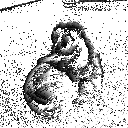
\includegraphics[width=0.3\textwidth]{puppyBall.png}
    \caption{A decayed image of a puppy with a ball}
\end{wrapfigure}
The simplest solution is to accumulate all the events in a given time slice into a 2D frame to recover images from the event-based data.
This is somewhat counter intuitive though as this forfeits all the temporal information which seperates the DVS from traditional cameras and results in a blury low resolution image. 
A method of preserving as much of the temporal information as possible is required. 


An approach to solve this problem is to choose a distinguished point in time, then construct a 2D image in which each pixels value is a function of its temporal distance to the distinguished point in time.
If only events that occured prior to the distiguished point in time are considered the resulting image would represent a faded history of what has just happened, this can be seen in figure \ref{fig:puppyBall} in which a recent history of the scene can be observed. 
Such images can be considered as a faded past, but are also known by many other equivilent names such as; temporal surface, decayed surface or time surface. 
There is no restriction as to why we must decay only into the past, a similarly interesting image can be produced decaying into the future from a distinguished point in time.
These decayed futures show where objects are moving to and can used as labels in a system trained to predict motion. 


The data is now in a form which can be used in traditional time-stepped neural networks and the temporal information has not been lost.
Still many questions remain to be explored such as what functions should be used to decay images and with what parameters.


\section{Function specifics and implementation}
%Include a quick maths wise description of this function\\
%Include some resulting images and discussion about each image as to why it is good or bad \\

The first and simplest decay function examined was linear decay. 
It can be characterised by equation \ref{eq:linearDecay}, intuitively in which the gradient (k) directly affects how much of the past (or future) is considered. 
Here $\Delta t$ is the temporal difference between the closest event for a given pixel and the distinguished point in time. 

% TODO why is this 1/k??

\begin{equation}
 \label{eq:linearDecay}
    f(\Delta t) = 
    \begin{cases}
    -\frac{1}{k}  \Delta t + 1 & 0\leq \Delta t \leq k \\
    0 & Otherwise
   \end{cases}
\end{equation}

An exponential function was also considered as a way to focus on only the most recent history.
Characterised by equation \ref{eq:expDecay} the length of history considered is dependent on the parameter k used. 

\begin{equation}
 \label{eq:expDecay}
    f(\Delta t) = exp\left(\frac{-\Delta t}{k}\right) \\
\end{equation}

To generate network inputs and outputs distinguished times must be selected and decayed around.
Each event in the event-stream could be used as a distinguished point and an input/output pair decayed around it.
This would generate a lot of redundant data as many similar events make up any given line.
Rather an event was selected at uniform time intervals to be decayed around.
A useful spacing was very problem dependent, interesting values to check were 10, 33 and 100 (\ms), unless otherwise specified 33\ms was used for this work so as to be similar to standard cameras. 
 


\subsection{Parameter influence}
Show some example parameters and how they affect the data \\


\section{Discussion}

 discuss the selections of k \\
 End up with a blur through time \\
 seems informative to humans at least? \\
 A little bit like a recurrent network (memory of past) \\



        % 4 
\chapter{Pilot study}
\label{ch:pilot}

%%%%%%%%%%%%%%%%%%%%%%%%%%%%%%      NET 1     %%%%%%%%%%%%%%%%%%%%%%%%%%%%%%%%%%%%%%
\section{pilotNet1}

%\subsection{Aims}

%\subsection{Method}

The first network created is intended to act as an exploration of the problem space to see what can be learnt and act as a benchmark for later models. 
It was designed to be simple to facilitate reasoning about it's internal dynamics with design decisions specified in table \ref{table:net1def}.
The weights for pilotNet1 were initialised with a truncated normal distribution with a standard deviation of $1 / ( number\_inputs * batch\_size )$ and the biases initialised to zero.
These weight values were chosen to be proportional to the network size and mini-batch sizes. 
Starting the biases at zero was chosen so each unit would consider it's inputs based solely on input weights initially and adjust the biases accordingly in training. 

\begin{table}[h]
\centering
\begin{tabular}{ | l | l | }
    \hline
    Num. Inputs & 16384 \\
    Num. Outputs & 16384 \\
    Connectivity & Fully connected \\
    Num. Hidden Layers & 1 \\
    Size Hidden Layer & 1, 2, 100, 16384  \\
    Activation function & Linear, ReLU, Sigmoid \\
    Loss & Sum Squared Error \\
    Learning rule & S.G.D. (back propogation) \\
    Learning rate & 0.001, 0.1, 0.5 \\
    Mini-batch size & 100 \\
    \hline
\end{tabular}
\caption{Features of net1}
\label{table:net1def}
\end{table}

% TODO discuss S.S.D loss function

Where each input/output corresponds to a single pixel in the decayed past/future.
Motivation to use one or two units in the hidden layer was derived from the linear nature of the dataset and the thought that the network may be able to model the data with just the gradient of the input.
The network was tested with both linear and non-linear activations to see if a non-linear layer was necesary.

\subsection{Results}
% TODO include some images from Net1 with input, label, output
The performance of the network on a validation set showed a initally rapid decrease follow by very steady decrease indicating the network has learnt the relatively simple task.
% TODO show sample outputs
However sample outputs from the network were all exactly the same regardless of the input and seemed to be a somewhat random pattern of activations.


\subsection{Discussion}
Results from this network highlighted some fundamental properties of the task that were not previously considered as well as some smaller issues with its own design.
Initialisation of the network weights using a standard deviation of $1 / ( number\_inputs * batch\_size )$ was reconsidered as this resulted in unecessarily small weights. 
As the network inputs are in the range [0-1] using a constant standard deviation of 0.1 is expected to give better results. 
Futher, initialisation of the biases to zero could have been causing ties during the back-progation phase and creating odd network dynamics.
To avoid this biases can be initialised just as weights with a normal distribution and standard devition of 0.1.

% TODO FInd the number of epochs (and include graph and reference)
Training the network with a learning rate of 0.001 showed a smooth decrease in the validation error over *** How many epochs *** epochs, increasing the learning rate resulted in a similar curve suggesting 0.001 was smaller than necessary to learn this simple pattern. 

These minor issues with network design were insignificant in comparison to an issue discovered with using the S.S.D. as a loss function. 
The sample predictions from the network are identical despite different inputs suggesting the network was learning something unexpected.
In any given input/output pair most ($>99\%$) of the input vector was zero or near zero meaning when computing the loss for a prediction the network could quickly achieve a small loss by simply outputting zero (or near zero) for every pixel regardless of what the input was. 
Pixels constant in the output correspond to 'hot pixels' in the DVS hardware, given they fire independently of other stimuli with their own frequency and location they constitute a sensible prediction for the model. 
The network achieved this by reducing the biases to the hidden layer isolating the output from the input.
It then used the weights from the hidden layer to the output to highlight the hot pixels based on each's frequency and keep the others off. 
%The network achieved this by simply reducing its biases with weights staying relatively stable meaning the input signal (the decayed trace of the dot's path) was lost as noise in the system. 


When running the network simulations it was abruptly clear that the network with 16384 hidden units was too large as the Tensorflow computation graph could not fit within the 12GB of memory on a single G.P.U.
The computation graph could be seperated onto multiple G.P.U.s to achieve results however this was considered unnecessary after discovering the problems associated with the loss function and considering the simple nature of the dataset.




%%%%%%%%%%%%%%%%%%%%%%%%%%%%%%      NET 2     %%%%%%%%%%%%%%%%%%%%%%%%%%%%%%%%%%%%%%
\section{pilotNet2}
After pilotNet1 some refinements were made although many of the features outlined in table \ref{table:net1def} were kept constant. 

Changes include:
% TODO Tidy up this list, the gaps are too large...
\begin{itemize}
    \itemsep-0.5em
    \item Weights initialised with standard deviation of 0.1
    \item Biases now initialised with normal distribution, standard deviation of 0.1.
    \item Added linear weighting to Loss function.
\end{itemize}

The pilotNet1 loss function suffered from each error the network made being equally weighted.
In any given image the vast majority of pixels should be predicted as near zero, while very few (roughtly 20) of the remaining pixels should be active. 
If the network mispredicts an \textit{on} pixel (that is a pixel which should be near one), this is a much more serious issue than if the network was to mispredict an \textit{off} pixel (a pixel that should be near zero). 
To minimise this issue a penalty could be applied to each type of mistake weighing incorrect active pixels (i.e. predicting one instead of zero) as only a small error while mispredicting an inactive pixel is considered a serious error.
Essentially penalising the network heavily for failing to predict the path of decayed pixels. 

\subsection{Weighted prediction penalty}
The weighting of penalty should be proportional to the activity in the input, such that if the signal is sparse then any mispredictions should be penalised heavily. 
% TODO Tidy up this maths and maybe take it out of line
If the activity is given by some variable $g$ then the penalty weighting for mispredicting a pixel as \textit{off} when it should be \textit{on} should be $(16384 - g) / 16384$, similarly a misprediction of a pixel as \textit{on} when it should be \textit{off} should only be $g / 16384$. 
In a system where neuron outputs were binary this would be all, however in the continuous output demmanded by a decayed representation inbetween values must be considered.
% TODO Add in linear equation and reference below
Interpolating linearly between these two points gives a general function to calculate how much weight a network mistake should be given, the function is shown in *** ref equation ***.
%In a binary system this would simply be a matter of weighing each  equation used is given in *** Ref equation *** 

% TODO Equation goes here

Including this weighting with the S.S.D. error function gives equation *** Ref full error fnctn***.

%TODO full error function goes here

\subsection{Results} 
% TODO get graphs and display


\subsection{Discussion}
Despite the various improvements offered over pilotNet1 this network still suffers from shifting weights and biases to generate a constant output regardless of the input. 
The signal to noise ratio of roughly $20/16384$ is to great to overcome with a simple linear weighting as specified above.
Perhaps the same tests with a larger dot which causes a greater number of events might be able to learn the pattern. 
Such an experiment is in some ways analogous to the work done in chapter *** ref attnetional networks chapter ***. 
Alternatively if the network could ignore large sections of the input and just search in smaller patches it may be able to extract some useful information.
This will be explored further in chapter *** REF convolutions ***. 

% TODO Consider moving to final discussion
The pilot study while unsuccessful in itself revealed interesting insight into the nature of the problem, primarily the signal to noise ratio and helped inform other network design decisions.
 




























             % 4
\chapter{Study 1 - Convolutional architectures}
\label{ch:convolutions}

%%%%%%%%%%%%%%%%%%%%%%%%%%%%%%      EVO Kernels    %%%%%%%%%%%%%%%%%%%%%%%%%%%%%%%%%%%%%%
\section{Evolutionary kernels}

\subsection{Aims}
%Tried to use evol kerns but sparse nature of data means no good
After the results from the Pilot study it was clear the task needed to be reframed.
Previous work using convolutions and kernels as feature detectors suggusted they might be able to provide feature maps necessary for a network to learn.
%Additonally using convolutions would have the advantage that they are able to ignore much of the image and focus on areas of activity.  
Convolutions may be well suited to this problem as they naturally focus on only small segments of the image meaning the signal-to-noise ratio affecting the PilotNets may be less problematic. 
Kernels capable of detecting dot motion were developed using an evolutionary algorithm. 
These dataset sepecific kernels were then used to transform the DVS recordings into feature maps in which each pixel represented the kernel for which it most highly responded. 
The feature maps were then used as training examples in a fully connected network with the aim being to analyse the performance of the network in predicting an output feature map. 
%Kenels specialised to the datasets were developed, these were then used to preprocess the input/output decayed images to produce feature maps which could then be used to train the network as per normal.
%Kernels  to the datsets were developed and then used to process recordings into training examples.

\begin{figure}[h]
    \centering
    \includegraphics[width=0.8\textwidth]{evoNetStructure.png}
    \caption{Structure of the Evolutionary Kernels processing pipeline}
    \label{fig:evoNetStructure}
\end{figure}

\subsection{Method}
Three major steps were required to convert from a DVS recording to a prediction in this study, the final system is illustrated in figure \ref{fig:evoNetStructure}.
First kernels for convolutions were evolved to be specialised to the 8AD dataset using a 1 + 1 hillclimbing algorithm (described in Appendix \ref{ch:evolution}). 
After sufficient evolution they were convolved with the DVS recording to produce feature map training examples.
The feature maps specifying which kernel had responded most strongly for that pixel were fed into a fully connected network which predicted future feature maps at the output.  

\begin{figure}[h]
    \centering
    \includegraphics[width=0.7\textwidth]{evoStableTrimmed.png}
    \caption{An example kernel evolution converging to a stable state}
    \label{fig:evoStable}
\end{figure}

\subsubsection{Evolving kernels}
As no standard set of feature kernels to use with event-based data exists these would need to be created.
Previous work developing kernels using an evolutionary algorithm made this a sensible place to start.
In this work a kernel is considered as a matrix with each value being a weight describing how important an event at that position is.
Kernels start randomly initialised and are iteratively updated by permuting kernel weights and convolving the new kernel with some sample data, improvements in kernel performance as measured by a fitness function are kept.
Figure \ref{fig:evoStable} shows what a kernel evolving from an initially random state (top row) looks like after 200 evolutionary steps (bottom row).
Each row in the image represents the kernels state at an evolution step while each column represents an individual pixels value at any step. 
A stable kernel signifies the kernel has found a local maximum in capturing information from a particular recording.
Finer details of the evolutionary algorithm are discussed in Appendix \ref{ch:evolution}.
A set of nine and a set of five kernels were created using this technique.
Motivation for using nine kernels was inspired by the 8AD dataset with anticipation that each kernel would specialise for one of the angles plus one kernel to detect noise.
Five was chosen to see if similar behaviour could be modelled as weighted combinations of less kernels.
A kernel size of 11x11 pixels was chosen as this would capture much of the temporal past (and future) for an accumulation over 33\ms.



\subsubsection{Processing training examples}
Convolving the 9, 11x11 kernels with the 128x128 images gave 9, 128x128 feature maps.
Rather than using pooling \textit{within} a feature map as is standard in convolutional neural networks max-pooling was applied \textit{between} the maps. 
That is the result was a single 128x128 map created in which each position was the index of the feature map with the highest output at that pixel.
An output feature map then represents which kernel the network predicts will be most active in any given pixel.
Using the output feature map in combination with the kernels a future temporal surface could then be reconstructed. 
%This decision was motivated by the idea that if the network learnt which kernels map to which a temporal surface prediction could be reconstructed using the output feature map with the kernels. 


\subsubsection{Network design} 
The networks used then resembled those of PilotNet2.
Representing each pixel as the kernel which most strongly responds to it should make predicting future motion simple task for a shallow network to learn.

\begin{figure}
    \centering
    \includegraphics[width=0.75\textwidth]{anaKerns.png}
    \caption{Example of four analytic kernels used}
    \label{fig:anaKerns}
\end{figure}

\subsubsection{Analytic kernels}
Additionally an alternative set of kernels was developed based on the probabilities of event patterns in the training data.
For all samples of a given angle an 11x11 matrix was cropped around each event, the probabilities of events in each position of the matrix was then calculated for that angle giving an analytic kernel.
The process of cropping an 11x11 matrix around events is the same process as discussed in Chapter \ref{ch:attentional}.
These kernels were significantly quicker to compute compared to the evolutionary kernels which required many convolutions of the full dataset for each evolution. 


\begin{figure}[h]
    \centering
    \includegraphics[width=0.7\textwidth]{evoUnstableInsert.png}
    \caption{(a) Non-converged evolution history for the final kernel shown in (b)}
    \label{fig:evoUnstableInsert}
\end{figure}

\subsection{Results}
Using the available evolutionary algorithm proved to be too slow to develop meaningful 11x11 kernels on the large 8AD dataset.
The kernels were not able to converge to a stable point after 14 days of training, example kernels are shown in \ref{fig:evoUnstableInsert}.
Kernels showed signs of moving towards appropriate features (e.g. higher activations along the South-West diagonal) but still needed more time to develop. 
The kernel states after 14 days were applied to the data regardless to see if meaningful results could be achieved. 
Kernels were evolved with integer values for weights but before use the values were mapped to the range 0 to 1.
After application to the data the network became input invariant as per the pilotNets. 
The analytic kernels, shown in figure \ref{fig:anaKerns}, were also substituted in place of the evolved kernels and the processing pipeline re-run to get the same input invariant results. 


\subsection{Discussion}
Developing kernels evolutionarily which would be specialised to the dataset proved to be too computationally expensive for the duration of this project. 
A faster algorithm could have been implemented but was considered out of scope meaning only premature kernels were used.
Analytic kernels offered a promising alternative to evolutionary algorithms being much faster to compute and resembling the 8 angles clearly.
However, the analytic kernels were also unable to produce meaningful results suggesting a deeper problem remains. 
The deeper problem may be that the network which is still taking all 16384 inputs is suffering from a signal-to-noise-ratio problem.

Using inter-layer pooling to generate a final feature map which has map indices from the previous layer as values may need to be reconsidered.
In this scenario there is no meaningful reason why the kernels should be ordered yet they will be given order by the process of using their indices.
Hypothetically if the North-East diagonal was index five, South-West was six and South-East was seven than the network would need some way of rationalising what a value of 5.5 or 6.5 meant. 
Ordering the kernels based on angle might be a start to solve this problem but does not leave room for a noise kernel, further, this solution does not generalise to other more complex problem sets.
Methods of encoding the kernels as one-hot vectors were investigated but no functional method was found. 
%Using feature maps as training examples for a fully connected network did not provide a suitable solution to produce meaningful predictions. 
%The networks consistantly learnt to ignore the input, shift biases and output zeros to minimise loss quickly. 


%%%%%%%%%%%%%%%%%%%%%%%%%%%%%%      CONVOLUTIONAL NN    %%%%%%%%%%%%%%%%%%%%%%%%%%%%%%%%%%%%%%
\section{convNet}
%Define it what did it learn and what happened.
%Alternative approach of using evol kerns on full image

\subsection{Aims}
The amount of time required to evolve kernels using the available evolutionary algorithm meant an alternative approach was necessary. 
Directly using a conventional convolutional network represented the logical progression after evolving kernels manually. 
The experimental design remained similar to the evolutionary kernels as described in figure \ref{fig:evoNetStructure}.
The difference being for this study the 128x128 temporally accumulated images were directly used as inputs to the network which was responsible for developing the kernels and feature maps and pooling was done spatially within a feature map rather than between feature maps.
This study should be able to leverage the advantages of convolution networks (e.g. focused feature detectors on smaller parts of the image) whilst still being trainable in reasonable time. 

\begin{table}[h]
\centering
\begin{tabular}{ | l | l | }
    \hline
    Num. Inputs & 16384 \\
    Num. Outputs & 16384 \\
    Num. Hidden Layers & 3 \\
    Fully connected & 64, 1024 units \\
    Layers & Convolutions -\textgreater pooling -\textgreater output \\
    Output Activations & Linear, Sigmoid, ReLU \\
    Loss & Sum Squared Difference, weighted S.S.D. \\
    Learning rule & S.G.D. (back propogation) \\
    Learning rate & 0.5 \\
    Convolution stride & 1 \\
    \hline
\end{tabular}
\caption{Features of convNet}
\label{tb:convNetdef}
\end{table}

%Rather than using an evolutionary algorithm to evolve kernels with which to later apply convolutions to the data this can all be done within a Convolutional Neural Network. 
%This network should be able to produce much of the behaviour of the evolved kernels (because it will be designing its own during training) but shouldn't suffer from the slow training time and possible inconsitancys between training and test data.

\subsection{Method}
\label{sec:convMethod}
The network used in this work consisted of an input layer followed by a convolution layer with 9, 11x11 convolutions followed by a 2x2 max pooling layer feeding into a fully connected layer. 
The output layer of the network was differently activated to compare performance. 
Details are outlined in table \ref{tb:convNetdef}.


\subsection{Results}
The convolution networks quickly (\textless 250 epochs) become input invariant.
This is shown in figure \ref{fig:convInputInvariance} in which despite a strong relatively clean signal the network is not able to make a meaningful prediction. 
The mechanism for this invariance can be seen in the weights and biases of the network over the first 5000 epochs.
The weights shift between 3 and -3 while the biases quickly shift towards -3, this example network (ReLU activated) then outputs just zeros.
This trend was consistant across the other convolutional architectures and parameters outlined in table \ref{tb:convNetdef}.

\begin{figure}[h]
    \centering
    \includegraphics[width=0.8\textwidth]{convNetInvariance.png}
    \caption{An example of a convolutional network input invariance and the corresponding fully connected layer features}
    \label{fig:convInputInvariance}
\end{figure}

\subsection{Discussion}
Convolutional architectures should have been well suited to solving this sparse signal problem.
The architectures used in this study were able to make any meaningful predictions and quickly learnt to just output a constant zero pattern much like like the PilotNets.
Several factors could have contributed to the poor performance of these networks including signal-to-noise ratio, number of epochs, learning rate or the training data. 

The convolutional networks were believed to have been better able to deal with the signal-to-noise ratio however the ratio may have proved still too high for the networks.
Convolution sizes were chosen to consider this with an 11x11 convolution resonably converying an accumulated past/future over a 33 ms window. 
An 11x11 area may have been too large yet the 6x6 kernels were not able to learn either suggesting there may still be other problems.
The noise in the training data may have proved problematic for learning. 
Each kernel may have specialised to pick up different kinds of noise and as noise is inherently unpredictable the kernels learn to predict zero. 

Networks were trained with 50,000 epochs which when compared with how quickly the network became input invariant was considered sufficient.
This number of epochs may not have been enough, perhaps the network needed more time to fine-tune the weights, this would be unlikely though given the lack of improvement in the first 50,000 epochs. 
The learning rate may have contributed to the network getting stuck in a local minima (outputting just zeros) and trying alternative learning rates may help the network learn.
Other techniques such a momentum \ref{sutskever2013importance} which can assist in learning may help but are left as future work.


% - Why did it perform so badly?? -> signal to noise, but even attentional convolutional fail later... Something inherent to convolutions?
 %- Was 1024 Units too many / not enough?
% - Were kernels comparable to evolved kernels / Analytic kernels?
% - How could this be improved?
% - Was the spacial max-pooling an influence




























      % 4
\chapter{Study 2 - Attentional Networks}
\label{ch:attentional}
To help simplify the learning problem the task was again reframed to improve the signal to noise ratio.
The preprocessing was adjusted such that frames were accumulated around every 150th event and instead of using the full image only an 11x11 frame was kept.
In keeping with previous experiments accumulation was applied into the past and future to be the input and output. 
Figure \ref{fig:11inoutpair} is an example of such a pair.
%Rather than applying decay to the whole image at uniform time intervals and using that as input the to the network each event was decayed around resulting in many more (albiet similar) training examples.
%However only an 11x11 area around each event was considered meaning the signal to noise ratio was much higher. 

\begin{figure}[h]
    \centering
    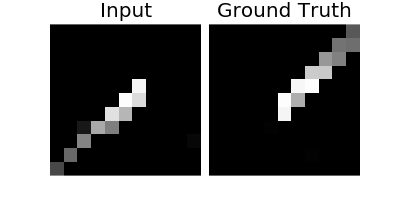
\includegraphics[width=0.8\textwidth]{11xinoutpair_83.png}
    \caption{Example of 11x11 input for an attentional network}
    \label{fig:11inoutpair}
\end{figure}

Figure \ref{fig:11inoutpair} is a cherry picked training example.
The Attentional networks still had a noisy task to solve because all events, including noise events, are considered. 
Many of the training examples derived from noise pixels could have been filtered out efficiently by demmanding the total activity in a training example excede some low threshold.
However, the system should be able to deal with noise and setting such a threshold would create another unnecessary hyper-parameter to the model.
Additonally such a parameter would be dependent on the time scale of the data and would need to be adjusted for each task. 
As will be shown the network was able to learn even in the midst of such noise so it was left in. 

%%%%%%%%%%%%%%%%%%%%%%%%%%%%%%      ATTENTIONAL NN    %%%%%%%%%%%%%%%%%%%%%%%%%%%%%%%%%%%%%%
\section{Attentional Directly Connected (ADC) Network}

\subsection{Aims}
% TODO Need to actually set some aims here
The network, as the name suggests, is a direct connection between the input and output units with no hidden layer.
The prediction problem had been broken down into a seemingly simple task so it was expected that results could be achieved with a simple network now the signal-to-noise ratio was larger within training examples.

\subsection{Method}
The network details are outlined in table \ref{tb:attnet1def}, with key points being the loss function has returned to the standard S.S.D. instead of the linearly weighted S.S.D. and the number of inputs has drastically decreased. 

\begin{table}[h]
\centering
\begin{tabular}{ | l | l | }
    \hline
    Num. Inputs & 121 \\
    Num. Outputs & 121 \\
    Connectivity & Fully connected \\
    Num. Hidden Layers & 0 \\
    Activation function & Linear, ReLU, Sigmoid \\
    Loss & Sum of Squares Difference \\
    Learning rule & S.G.D. (back propogation) \\
    Learning rate & 0.1 \\
    Mini-batch size & 100 \\
    \hline
\end{tabular}
\caption{Features of the Attentional Directly Connected Networks}
\label{tb:attnet1def}
\end{table}

\subsection{Linear activation}
The simplest ADC network considered had only a linear activation to compute outputs. 
This proved to be enough for the network to learn to make coherent predictions. 
The two datasets (8 Angle and Arbitrary Angle) were considered, a network was trained on each and then made predictions on a set of validation data from it's own dataset and other dataset to see how it could generalise.
For clarity the networks trained on the 8AD will be called 8AngNets and the networks trained on the AAD will be called ArbAngNets. 

\subsubsection{Linearly activated 8AngNet results}

\begin{figure}
    \centering
    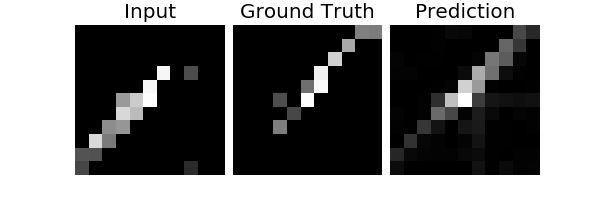
\includegraphics[width=0.8\textwidth]{ADC_8a_8a_13.png}
    \caption{A reasonable prediction from 8AngNet on the 8AD validation set.}
    \label{fig:ADC_8a_8a_crct} 
\end{figure}

\begin{figure}
    \centering
    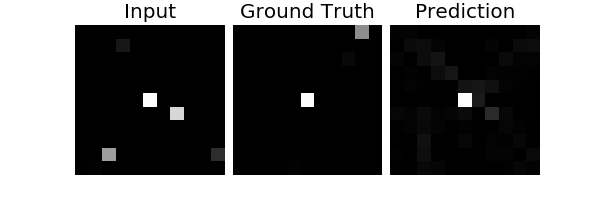
\includegraphics[width=0.8\textwidth]{ADC_8a_8a_7.png}
    \caption{A prediction from 8AngNet with a noisy input}
    \label{fig:ADC_8a_8a_noisy}
\end{figure}

Figures \ref{fig:ADC_8a_8a_crct} and \ref{fig:ADC_8a_8a_noisy} show how the linearly activated 8AngNet predicted in two cases from the 8 Angle validation set.
This prediction looks promising that the network is capable of representing some structure of the data as the prediction is similar to the label (ignoring some noise).
% TODO Make this an even more correct image and use this particular img (13) later to discuss problems
%In figure \ref{fig:ADC_8a_8a_crct} the network is performing well and gives a prediction which is quite similar the ground truth (ignoring noise). 
Figure \ref{fig:ADC_8a_8a_noisy} shows a noisy training example.
The label does not intuitively follow from the input and the network only outputs small values.
However the network does predict faintly along the North-West diagonal which is sensible when considering the input has two pixels along the South-East diagonal (the closer of which is highly active making it resemble a decayed path). 
%However the network has noticed two pixels active along the bottom right diagonal (one of which is highly active) and the network predicts a faint output along the top left diagonal.

\begin{figure}
    \centering
    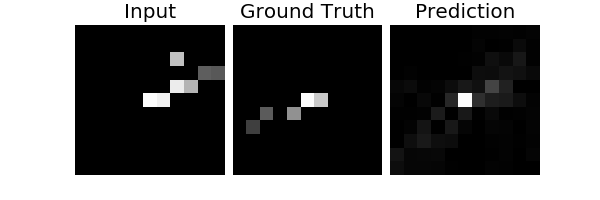
\includegraphics[width=0.8\textwidth]{ADC_8a_aa_4.png}
    \caption{8AngNet struggles to predict AAD examples}
    \label{fig:ADC_8aNoaa}
\end{figure}

\begin{figure}
    \centering
    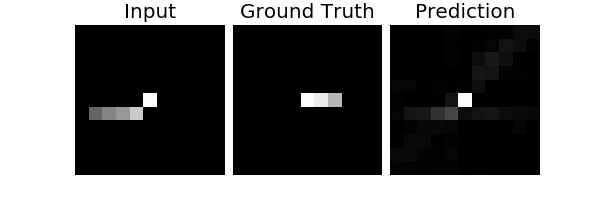
\includegraphics[width=0.8\textwidth]{ADC_8a_aa_46.png}
    \caption{8AngNet predicting a slightly off angle input}
    \label{fig:ADC_8aNoaa_fork}
\end{figure}

The network performing well on its own validation set is a success in itself but raises the question of how it will generalise from 8AD to AAD.
It was hypothesised the network might be able to use a combination of known angles to represent the new angles in the Arbitrary Angle dataset.
This was not the case though, figure \ref{fig:ADC_8aNoaa} shows the network stuggling to predict the motion.
Most of the activity in the prediction falls in the East North-East section which is where the input was.
There is some very limited activity that matches the label but this is insignificant compared to previous predictions and what can be realistically expected from the network. 
Further figure \ref{fig:ADC_8aNoaa_fork} shows a slightly off center input which resembles an angle from 8AD. 
The network has trouble interpreting this and makes 3 very faint predictions being the North-East diagonal, the East edge and along the input.
This suggests the network is not able to efficiently represent the arbitrary angles as some combination of the angles it learnt and must be using some other internal representation such as mapping between regions.

An additional interesting case which supports a region mapping hypothesis is seen in figure \ref{fig:ADC_8aNoaa_special} in which the network suffering from some neatly aligned noise. 
The network is well equipped to deal with inputs coming from one angle at a time but this noise makes it appear as if two dots may be crossing paths. 
The networks behaviour to predict two strong output paths shows that each input path (and its predictions) are happening (at least somewhat) independently of the rest of the input.
If the network was representing the input as an angle it would be reasonable to expect that the output might be a blur in the North-East corner of the prediction.  
Instead this clear prediction of two paths suggests the network is simply learning to map between areas of the input to areas of the output. 

\begin{figure}
    \centering
    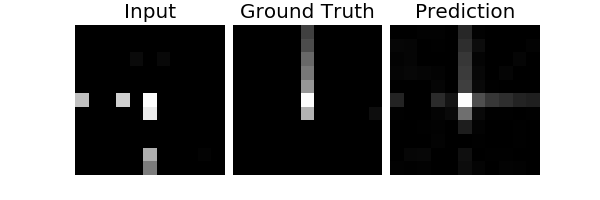
\includegraphics[width=0.8\textwidth]{ADC_8a_aa_15.png}
    \caption{8AngNet network predicting two paths due to noise}
    \label{fig:ADC_8aNoaa_special}
\end{figure}


\subsubsection{Linearly activated ArbAngNet results}
It follows that a network trained on only 8 angles would have trouble generalising to arbitrary angles so a second network was trained on the Arbitrary Angles Dataset. 
In general the network trained on Arbitrary Angle data was less confident in its predictions (magnitude of predictions were lower) but in each guess it would cover a boarder area. 
% TODO rewrite this sentence
An example of this is figure \ref{fig:ADC_aaaa_crct} in which the prediction has many faintly coloured squares, in contrast to the more confident predictions made in figure \ref{fig:ADC_8a_8a_crct} by 8AngNet.

\begin{figure}[h]
    \centering
    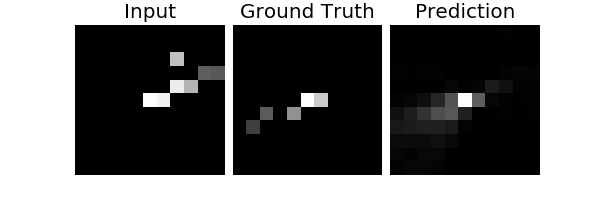
\includegraphics[width=0.8\textwidth]{ADC_aa_aa_4.png}
    \caption{ArbAngNet correctly predicting}
    \label{fig:ADC_aaaa_crct}
\end{figure}
% TODO these visualisations can be improved by grouping the predictions from both nets into 1 img


\begin{figure}[h]
    \centering
    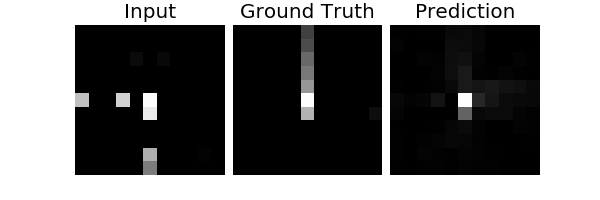
\includegraphics[width=0.8\textwidth]{ADC_aa_aa_15.png}
    \caption{ArbAngNet predicting two paths due to noise}
    \label{fig:ADC_aaaa_twopath}
\end{figure}

\begin{figure}[h]
    \centering
    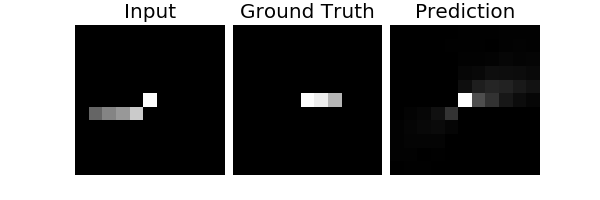
\includegraphics[width=0.8\textwidth]{ADC_aa_aa_46.png}
    \caption{ArbAngNet predicting a slightly off angle input}
    \label{fig:ADC_aaaa_fork}
\end{figure}


The neat noise example which suggested that 8AngNet was simply mapping regions in the input to regions in the output shows a very different prediction from ArbAngNet.
ArbAngNet does not predict any given angle strongly but instead has a very faint prediction along both but also between the two lines. 
The significance of these prediction is questionable given how small the predictions are but it does give some insight into the networks dynamics.
It should be noticed that this does not exclude the possibility that ArbAngNet is also just mapping between regions of the input and output, rather this is still a promising theory.
Finally, figure \cite{fig:ADC_aaaa_fork} shows ArbAngNets performance on the slightly off angle example that 8AngNet failed to predict in figure \ref{fig:ADC_8aNoaa_fork}.

\subsection{Non-linear acitivation}
Compare Sigmoidal with relu?

\subsubsection{Sigmoid activation}
Talk about both 8AD and AAD here

\subsubsection{ReLU activiation}
Talk about both 8AD and AAD here 

\subsection{Attentional Directly Connected network discussion}
The ADC networks were successfully able to make meaningful predictions on both the 8AD and AAD datasets even with only a linear activation.
Neatly aligned noise suggests the networks internal representation is to map between pixels in the input to pixels in the output.
This is supported by 8AngNets inability to generalise to the AAD, naturally if the network hasnt learnt that a region (i.e. between two angles of 8AD) should map to another region than it will not be able to generalise to this. 
If the network had learnt to represent the training examples as angles then this generalisation should have been possible. 


%%%%%%%%%%%%%%%%%%%%%%%%%%%%%%      ATTENTIONAL NN    %%%%%%%%%%%%%%%%%%%%%%%%%%%%%%%%%%%%%%
\section{Attentional Hidden Layer (AHL) Network}

\subsection{Aims}
Following in the 

 using a hidden layer, what can learn? maybe line params, 1, 2, more hiddens

\subsection{Method}

\begin{figure}[h]
    \centering
    \includegraphics[width=1\textwidth]{AHLrelu.png}
    \caption{ReLU activated AHL network performance with varying hidden units}
    \label{fig:attnConvInvariant}
\end{figure}

\subsection{Results}


\subsection{Discussion}

%%%%%%%%%%%%%%%%%%%%%%%%%%%%%%      CONV NET    %%%%%%%%%%%%%%%%%%%%%%%%%%%%%%%%%%%%%%
\section{Attentional convolutional networks}
\subsection{Aims}
With positive results from the ADC and AHL networks the possibility of the convolutional networks with the attentional training datasets was considered. 
The simple, regular structure in the attentional training data might be enough for a shallow convolutional network to learn. 

\subsection{Method}
The network structure, methodology and manipulated variables were identical to that in section \ref{sec:convMethod} with some minor differences.
These differences included the change in input/output size from 16384 to 121 and convolution size from 11x11 to 6x6. 
The input/output layer size change was necessary given the smaller size of the training examples and the convolution size change was considered given the input was now only 11x11.
As the attentional accumulation trims the training examples to 11x11 then in theory each temporal past/future should only take up a 6x6 grid. 

\subsection{Results}
Despite the attentional data and the reduced size the convolutional networks still become input invarient as shown in figure \ref{fig:attnConvInvariant}.
The activity pattern shown is from the network using a size 8 dot moving with speed 4 accumulated with an exponential function and k value corresponding to a 33 ms period.
This invariance was consistant (although the given activity pattern would change) regardless the number/size of feature maps, the fully connect layer depth and fully connected layer activation.

\begin{figure}[h]
    \centering
    \includegraphics[width=0.7\textwidth]{attConvInvariance64.png}
    \caption{Attentional Convolutional Net showing input invariance.}
    \label{fig:AHLrelu}
\end{figure}

\subsection{Discussion}
The cause for this invariance in not known, the most promising explaination being a problem similar to the invariance seen in the PilotNets.
That is that the network quickly learns it can minimise the loss function by setting most values to zero and highlighting pixels based on frequency of appearing in the output.
For the PilotNets the frequent pixels were the hot pixels, for the attentional convolutional networks the frequent pixels are those near the center.
This explaination has trouble explaining why the convolutional networks would be unable to learn using the S.S.D. loss function when the ADC and AHL networks are able to make meaningful predictions using it.  

%%%%%%%%%%%%%%%%%%%%%%%%%%%%%%      AUTO ENCODE     %%%%%%%%%%%%%%%%%%%%%%%%%%%%%%%%%%%%%%
\section{Auto Encoder}
\subsection{Aims}
Noise has been accepted as a fact of neuromorphic sensors so far in this work and models have been expected to be able to deal with this.
A simple thresholding could have efficiently filter out many of the noise based training examples before use in training. 
Such a threshold would be dataset specific (with larger/faster dots creating more events) though and creates an unnecessary hyperparameter to the model. 
Instead noise could be filtered out using an Autoencoder.
This possibility is explored with autoencoders of various size.

\subsection{Methodology}
Simple Autoencoders consisting of a single fully connected hidden layer were used. 

\subsection{Results}

\begin{figure}[h]
    \centering
    \includegraphics[width=0.85\textwidth]{AEUnits.png}
    \caption{Effects of additional hidden units on AAD dataset Autoencoder}
    \label{fig:AEUnits}
\end{figure}


\subsection{Discussion}
 
       % 8
%\chapter{Neural Networks}

\section{Net1}
Define the network, what was it, what was it meant to learn

\section{Net2}
Define it, why was it an improvement on net1?

\section{Evolutionary kernels}
Tried to use evol kerns but sparse nature of data means no good

\section{convNet}
Define it what did it learn and what happened.
Alternative approach of using evol kerns on full image

\section{Attentional Networks}
Zooming in around the most current event

\section{Auto Encoder}
How much could be cleaned up
Retry other networks with cleaned up data. 



       
\chapter{General discussion and conclusions}

\section{Major findings}
The studies in this work show that neural networks were able to make meaningful predictions of temporal surfaces.
These predictions could be achieved with a single linearly activated output layer which demonstrates how readily available temporal information is in temporal surfaces.
Using deeper networks with a single hidden layer reduced the performance of the predictions in some cases, due to the network being forced to represent the stimulus with the number of units in the hidden layer (typically less than the input). 
Convolutional networks which were expected to be able to deal well with the full scene temporal surfaces became input invariant even with the attentional surfaces.
This result, in light of the simpler networks' learning, suggest the problem may be with the convolutional structure used in these studies and that other structures may be able to produce meaningful predictions.
Autoencoders were shown to be able to smooth out the input data and may be useful in future work where noise is a concern. 
None of the examined networks were able make meaningful predictions directly using the full scene temporal surfaces.
However a demonstration of how attentional surfaces can be used to recreate full scene predictions is also presented. 

Additional insights from the research found little difference between using a linear or exponential accumulation function. 
Linear had fewer but more highly active pixels, while exponential had a longer accumulation tail but also retained noise pixels for longer.
All major trends in terms of network performance were found with both accumulation functions.
Similarly the dot size and speed had no influence on the overall trends of network performance. 
Together, testing these parameters (function, speed and size) contributed to a 24 times increase in number of networks run and over compute power/time used. 
It was found that the constant used in the accumulation function did impact the performance of the network.
Such an impact is expected; as the amount of time in a given accumulation period decreases so does the amount of past information available to the network to learn from. 
A requirement of a given time period to make meaningful predictions does not exclude this kind of processing from realtime systems 
The time period required can be used as a sliding window so processing can be done at any time based on the last time period worth of information. 

% Move 4a & 3b - impact of the results on the aims
It has been demonstrated that frame-based shallow neural networks are able to leverage implicitly encoded temporal information to make meaningful predictions of future temporal surfaces. 
These successful predictions suggest that temporal surfaces are capable of implicitly encoding temporal information and that frame-based neural networks are able to leverage it meeting the aims of this work. 
A general result from this work being verification of the functionality of temporal surfaces as an intermediary between event-based vision sensors and frame-based neural networks in simple cases such as linear motion. 
%While it does not seem like the networks were able to learn abstract features such as representing the data as angles they were able to make meaningful predictions from implicitly encoded 
Using temporal surfaces brings neuromorphic sensors one step closer to state-of-the-art vision processing techniques. 
While long term gains from neuromorphic hardware will come from the development of purpose built algorithms, short term gains in vision processing may come from representations such as temporal surfaces.  


\section{Possible future work}
A natural expansion on this work would be to validate the use of temporal surfaces with more complex datasets and networks. 
An initial starting point would be to use the multi-dot datasets to verify if results generalise to these cases.
A particular direction for this would be to apply temporal surfaces to real world dataset like robot motion such as those in \cite{Gibson2014, barranco2016dataset}. 
More complex networks may be required to extract visual features and as such further network design is a future direction for projects in this area. 
Convolutional networks which traditionally do very well with 2D images performed poorly in this work.
This poor performance is likely due to a network structure weakness or problem with the loss function. 
Exploring the difference between expected and actual performance may yield insight into the problem and a solution. 

During this work only a single time scale was considered in an experiment, a complex visual system would likely operate with a hierarchy of spatial and temporal scales.
A system of processing modules working simultaneously analysing temporal surfaces with different spatial (attentional size) and temporal scales (accumulation function constant size) might be able to extract complex real world features. 
Using a high-speed event-based sensor rather than a frame-based sensor would give this system the ability to process events according to some metric (based on previous processing or metrics of the events coming in) rather than uniformly as required by frame-based systems. 
The system could leverage the feature extraction ability of frame-based models with temporal freedom of the frame-free vision sensors.









        
%\chapter{Conclusions}

\section{Findings}

\section{Implications}

\section{Possible future work}

       % 4 



%%%%%%%%%%%%%%%     REFERENCES    %%%%%%%%%%%%%%%%%
%\begin{thebibliography}{99}
%\addcontentsline{toc}{chapter}{References}
%\bibitem{lamport} L.~Lamport, \emph{\LaTeX: A Document Preparation
%System}, 2nd ed. (Addison-Wesley, 1994).
%\bibitem{LABEL2} REFERENCE 2
%\bibitem{ETC.} Etc.
%\end{thebibliography}

\bibliographystyle{IEEEtran}
\bibliography{/home/joti/Documents/References/mendeley_bibs/thesis}



%%%%%%%%%%%%%%%%%    APPENDIX    %%%%%%%%%%%%
\appendix
% Chapters after the \appendix command are lettered, not numbered.
\newpage
\mbox{}
\newpage

% \include appendix chapters here.

\chapter{Evolutionary Kernel Algorithm}
\label{ch:evolution}

\textbf{NOTE: The work described in this section was completed by the author during a seperate reserach project.}

A 1+1 evolutionary hill climber algorithm was used to competitively train a number of initially random kernels on event-based data.
The DVS data was discretised as a 3D grid in which a voxel was assigned a value of 1 if any event occurred or a placeholder value (-1/27) otherwise.
The small negative weight was chosen as a penalty when the kernel highlights an area with no events.
The value of -1/27 is kept from previous work upon which this method is based and has no significance to this project but is kept for it's properties as a penalty. 
Kernels were constrained to be zero sum during training and individual elements were limited to the range of -27 to 27.
The range is also from previous work and arbitrarily kept as the specific values used will have little impact on the structure of evolution. 
During evolution only positions in which the centre of the kernel was on an event were included in calculations so that kernels could specialise to centered events rather than trying to capture features with the edges of the kernel. 
At each evolution the champion from the previous evolution step and its mutant were scored against the other champions from the previous evolution.
If the mutant performed better by a fitness function it was considered the champion for that evolution step otherwise the champion would remain. 
Only one mutant was tried per kernel at each step of evolution.

\section{Selection algorithm}
The selection function used describes how well a kernel performs on some data. 
In this work the kernel was assigned the value of the sum of its output on each event in which it was the highest scoring kernel out of the competitors. 
A biological analogy being the sum of the calories in all of the meals the kernel won. 
Only rewarding a kernel when it ‘wins’ an event helps the kernels niche out sections of the data. 
Then once niched they can continue to specialise to that niche by maximising their output (calories) on the events they have won. 

\section{Mutant operations}
A mutation could include, two zeros being made to a -1 and 1 (or vice-versa) or two elements may be selected at random and have +1 and -1 added to them. In practise the kernels quickly removed any ones or zeros so the only mutation applied was that of randomly incrementing and decrementing elements. This proved a flexible algorithm that allowed a kernel to escape from mistakes it makes. Using smaller or more proportional changes may have resulted in different behaviour however this wasn’t explored widely. 



%\chapter{Tensorboard network structures}
\label{ch:tbnets}

This appendix will hold tensorboard images of each network for reference
\section{Net1}
\section{Net2}
\section{Evolutionary Kernels network}
\section{convNet}
\section{Attentional Network}
\section{AutoEncoder}


\cleardoublepage


\end{document}
